% Intestazione
\fancyhead[L]{3 \hspace{0.2cm} Modello di sviluppo} % Testo a sinistra

% Sezione 
\section{Modello di sviluppo}
\label{sec:modello_sviluppo}
Un modello di sviluppo è un approccio strutturato per organizzare, pianificare e gestire le diverse fasi di creazione di un software.\\
È stato scelto, in conformità con il proponente, il modello \emph{Agile}\textsubscript{\textit{\textbf{G}}} per la sua capacità di adattarsi ai cambiamenti e per l’approccio iterativo e incrementale, che consente di migliorare il software attraverso cicli brevi chiamati sprint.\\
Il metodo promuove la collaborazione continua con il cliente e il feedback frequente, facilitando l’identificazione rapida di eventuali modifiche necessarie e riducendo il rischio di problemi significativi alla fine del progetto.\\

\subsection{Lo Standard ISO/IEC/IEEE 12207}
L'\emph{ISO/IEC/IEEE 12207}\textsubscript{\textit{\textbf{G}}} definisce un \emph{framework}\textsubscript{\textit{\textbf{G}}} completo per il ciclo di vita del software, identificando processi, attività e compiti necessari per sviluppare, gestire e mantenere software in modo sistematico. Implementare questo standard permette di mantenere un alto livello di qualità, tracciabilità e coerenza nei processi di sviluppo software. Fornisce un quadro di riferimento robusto per gestire i progetti, favorendo il miglioramento continuo e il rispetto delle tempistiche e dei requisiti iniziali.\\
Lo standard si articola in tre principali categorie di processi:
\begin{itemize}
    \item Processi primari
    \item Processi di supporto
    \item Processi organizzativi
\end{itemize}

\subsubsection{I processi primari}
I processi primari comprendono quelli necessari alla gestione e allo sviluppo del software, includendo sia la gestione del progetto sia il supporto tecnico.
\begin{itemize}
    \item \textbf{Processo di acquisizione}: Coinvolge tutte le attività di acquisizione del software o di servizi legati al software, come la definizione dei requisiti dell'acquirente, la selezione del fornitore, la gestione del contratto e il monitoraggio del progresso.
    \item \textbf{Processo di fornitura}: Descrive le attività del fornitore per sviluppare, modificare e consegnare il software in base alle specifiche di contratto. Include la pianificazione, lo sviluppo, la consegna e la gestione del software.
    \item \textbf{Processo di sviluppo}: Definisce le attività per creare o modificare il software. Le fasi principali sono:
    \begin{itemize}
        \item \textbf{Analisi dei requisiti}: Identificazione delle specifiche funzionali e non funzionali.
        \item \textbf{Progettazione del sistema e del software}: Progettazione dell'architettura e della struttura del software.
        \item \textbf{Implementazione}: Programmazione del codice sorgente.
        \item \textbf{Integrazione}: Assemblaggio delle diverse parti del software.
        \item \textbf{Testing}: Verifica del software per assicurare che rispetti i requisiti definiti.
        \item \textbf{Installazione e accettazione}: Rilascio del software e conferma della sua aderenza ai requisiti.
    \end{itemize}
    \item \textbf{Processo di gestione operativa}: Si occupa delle attività di gestione del software nel suo ambiente di produzione, incluse la manutenzione, il supporto utente, l'operatività continua e il monitoraggio delle performance.
    \item \textbf{Processo di manutenzione}: Comprende tutte le attività per correggere, migliorare o adattare il software dopo il rilascio, al fine di mantenerne o aumentarne l'efficienza e la rilevanza.
\end{itemize}

\subsubsection{I processi di supporto}
Questi processi assistono i processi primari e garantiscono che il software sia conforme agli standard di qualità.
\begin{itemize}
    \item \textbf{Processo di documentazione}: Definisce la creazione, la gestione e la manutenzione della documentazione di progetto.
    \item \textbf{Processo di configurazione}: Gestisce le versioni del software, tenendo traccia delle modifiche e assicurando che ogni versione sia stabile e rintracciabile.
    \item \textbf{Processo di verifica}: Garantisce che ogni fase dello sviluppo rispetti i requisiti iniziali attraverso attività di verifica e review, che coinvolgono sia il codice che la documentazione.
    \item \textbf{Processo di validazione}: Assicura che il software finale soddisfi le esigenze dell'utente, attraverso attività di testing e collaudo in condizioni reali.
    \item \textbf{Processo di garanzia di qualità}: Definisce le attività di controllo qualità per monitorare la conformità agli standard e migliorare continuamente i processi di sviluppo.
    \item \textbf{Processo di revisione e audit}: Prevede revisioni periodiche e audit di progetto per identificare eventuali problemi o non conformità rispetto agli standard definiti.
\end{itemize}

\subsubsection{I processi organizzativi}
I processi organizzativi mirano a sostenere e migliorare i processi aziendali nel loro insieme, creando un ambiente di supporto che faciliti l'attività dei team.
\begin{itemize}
    \item \textbf{Processo di gestione}: Include tutte le attività di pianificazione, coordinamento e monitoraggio del progetto, come l'assegnazione delle risorse, la definizione del budget e la gestione del rischio.
    \item \textbf{Processo di miglioramento}: Riguarda le attività di analisi e ottimizzazione dei processi, come la raccolta di feedback, l'identificazione delle aree di miglioramento e la messa in atto di strategie di ottimizzazione.
    \item \textbf{Processo di formazione}: Definisce la formazione continua per il personale, migliorando le competenze tecniche e manageriali necessarie a svolgere i vari processi.
    \item \textbf{Processo di gestione delle risorse umane}: Include le attività di selezione, valutazione e gestione delle risorse umane impiegate nei vari processi.
\end{itemize}

\newpage

\subsection{Struttura dello Sprint Agile in conformità con lo Standard ISO/IEC/IEEE 12207}
In Agile, l'approccio si basa sull'evoluzione continua del prodotto attraverso iterazioni brevi, chiamate \emph{sprint}\textsubscript{\textit{\textbf{G}}}, in cui vengono rilasciate nuove funzionalità incrementali.\\
Ogni sprint produce un incremento funzionante del prodotto, che viene migliorato e raffinato nelle fasi successive. L'approccio Agile si concentra sulla collaborazione costante con il cliente e sull'adattamento alle sue esigenze, dando priorità ai requisiti più rilevanti e adattabili. L'obiettivo è fornire il prodotto il più rapidamente possibile, con versioni utilizzabili fin da subito, migliorandolo progressivamente attraverso feedback continui.\\
L'immagine in figura \bulref{fig:Struttura di uno Sprint Agile della durata di due settimane} mostra la struttura di uno Sprint Agile della durata di due settimane, scelta in comune accordo con il proponente.\\
\begin{figure}[h] 
    \centering
    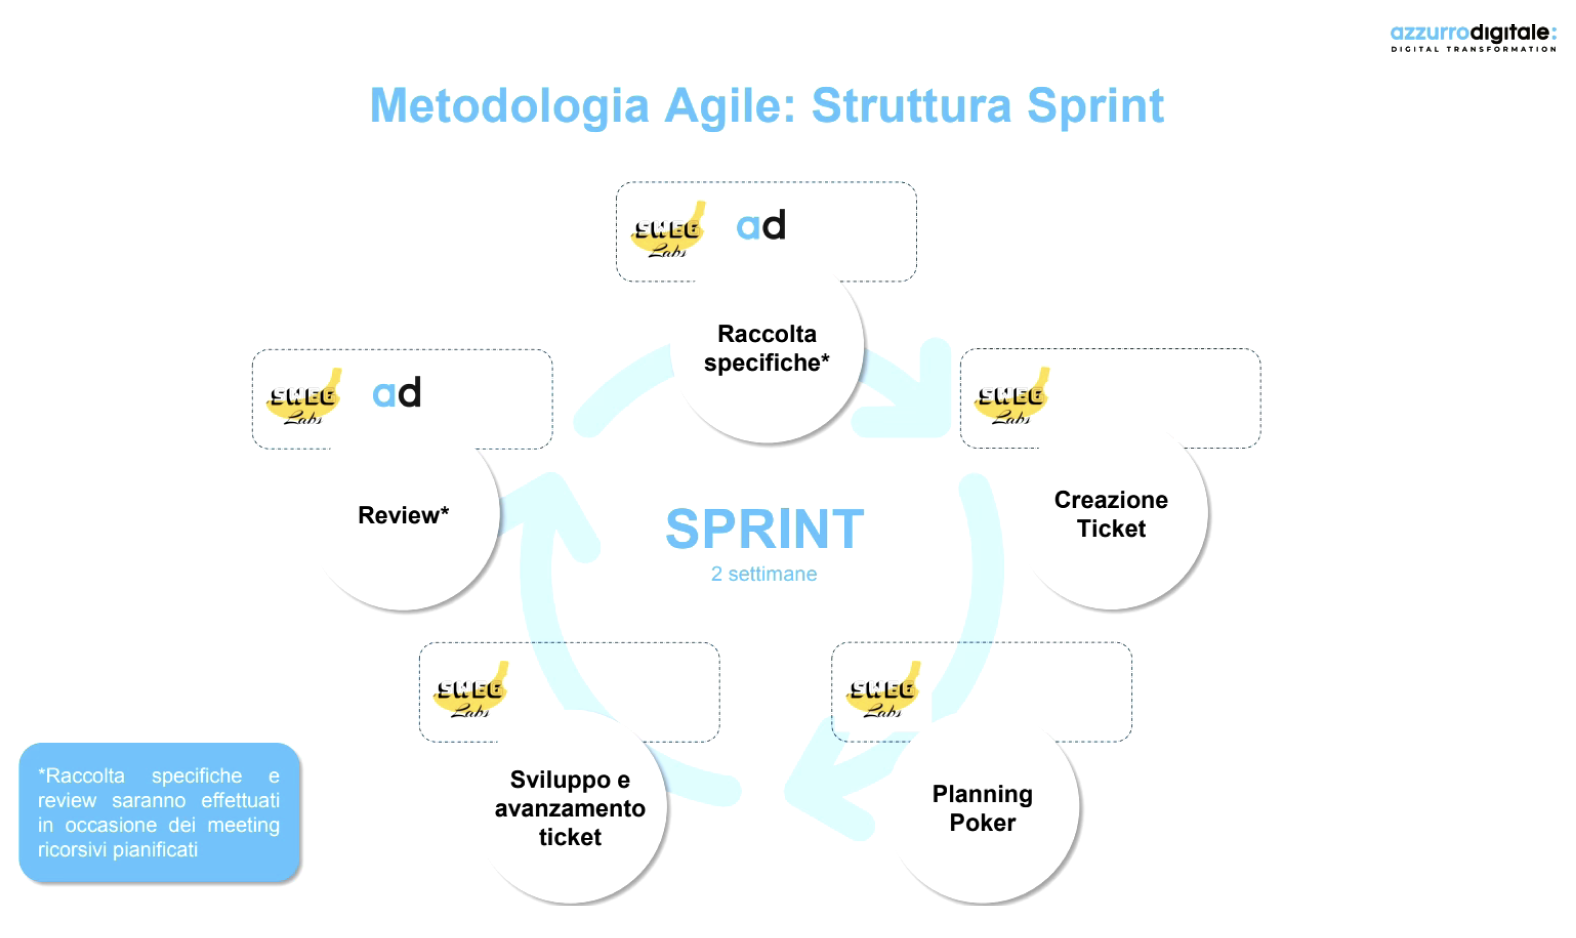
\includegraphics[width=\textwidth]{Sprint Agile.png}
    \caption{Struttura di uno Sprint Agile della durata di due settimane} 
    \label{fig:Struttura di uno Sprint Agile della durata di due settimane}
\end{figure}

Di seguito, viene spiegato come questo processo può essere visto alla luce dello standard ISO/IEC/IEEE 12207.
\begin{itemize}
    \item \textbf{Raccolta Specifiche}: Nella metodologia Agile, questa fase corrisponde alla raccolta dei requisiti attraverso incontri ricorsivi e interazioni frequenti con gli stakeholder, così come suggerito nello standard ISO/IEC/IEEE 12207 tramite il Processo di acquisizione. Qui vengono definiti i requisiti iniziali e i cambiamenti necessari per soddisfare le aspettative.
    \item \textbf{Creazione Ticket}: Questa fase rappresenta l'organizzazione dei requisiti e la suddivisione del lavoro in compiti specifici o "ticket". Nell'ISO/IEC/IEEE 12207, questa attività si allinea al Processo di sviluppo, dove la progettazione e la definizione dei task facilitano la realizzazione incrementale del progetto.
    \item \textbf{Planning Poker}: Durante il planning poker, il team stima lo sforzo richiesto per ciascun ticket. Questo è legato al Processo di gestione previsto dallo standard, che include attività di pianificazione delle risorse, assegnazione dei ruoli e previsione dei tempi.
    \item \textbf{Sviluppo e avanzamento ticket}: Questa è la fase in cui il lavoro viene svolto sui ticket, con sviluppo, implementazione e testing. Rientra nel Processo di sviluppo dell'ISO/IEC/IEEE 12207, dove si affrontano implementazione e integrazione del software.
    \item \textbf{Review}: La fase di review consente al team di valutare il lavoro svolto e raccogliere feedback sugli incrementi prodotti. Questo riflette i Processi di verifica e validazione dello standard ISO/IEC/IEEE 12207, assicurando che il software soddisfi i requisiti e sia conforme agli standard di qualità.
    \item \textbf{Sprint Review e Raccolta Specifiche per il ciclo successivo}: Come evidenziato nell'immagine, la fase di raccolta specifiche e review sono attività iterative che si svolgono durante i meeting ricorsivi. Questi incontri di retrospettiva permettono di raccogliere feedback, aggiustare il lavoro futuro e migliorare i processi, allineandosi al Processo di miglioramento dello standard, che mira all'ottimizzazione continua dei processi e alla qualità del prodotto.
\end{itemize}

    
   
    






